\chapter{User guided synthesis}
\label{ch:userguided}

This chapter formalizes the device driver synthesis problem using two player games. It then presents the Termite device driver synthesis toolkit which builds on this formalism to create a practical driver synthesis tool.

\section{Introduction}\label{sec:user_guided_intro}

\subsection{Overview of \termite} Figure~\ref{f:termite} gives an overview of the driver synthesis process, described in detail in the rest of this chapter.  \termite takes three specifications as its inputs: a device model that simulates software-visible device behavior, an OS model that specifies the software interface between the driver and the OS, and a driver template that contains driver entry point declarations and, optionally, their partial implementation to be completed by \termite.

\begin{figure}
    \center
    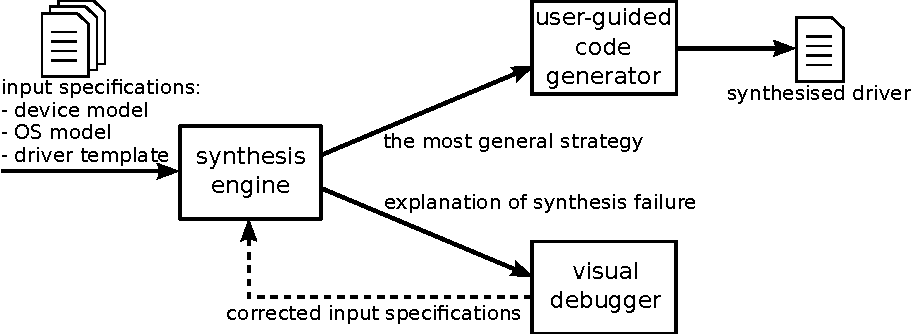
\includegraphics[width=\linewidth]{imgs/termite.pdf}
    \caption{\termite synthesis workflow.}\label{f:termite}
\end{figure}

Given these specifications, driver synthesis proceeds in two steps.  The first step is carried out fully automatically by the \termite game-based synthesis engine, which computes \emph{the most general strategy} for the driver---a data structure that compactly represents all possible correct driver implementations.  This step encapsulates the computationally expensive part of synthesis.  At the second step, the most general strategy is used by the \termite code generator to construct one specific driver implementation in C with the help of interactive input from the user.

The synthesis engine may establish that, due to a defect in one of the input specifications, there does not exist a specification-compliant driver implementation.  In this case, it produces an explanation of the failure, which can be analysed with the help of the \termite debugger tool in order identify and correct the defect.

%        order to help the developer identify and correct the 
%        defect, the synthesis engine generates a data structure, 
%        called \emph{counterexample strategy}, representing device 
%        and OS behaviour that exposes the defect.  The driver 
%        developer uses the \termite visual debugger tool 
%        (Section~\ref{}) to explore the counterexample strategy, 
%        identify and correct the defect.  
        
%    \item We present the design an implementation of \termite in 
%    a top-down fashion.  We first explore the tool from the 
%    user's perspective.  
%
%        how input specifications for driver synthesis are created
%        
%        next, we explain how the user interacts with the \termite 
%        code generator to produce a well structured driver 
%        implementation.
%        
%        Next we look under the hood

\subsection{Limitations of \termite}  The device driver synthesis technology is still in its early days and, as such, has several important limitations.  Most notably, \termite does not currently support synthesis or verification of code for managing direct memory access (DMA) queues.  This code must be written manually and is treated by \termite as an external API invoked by the driver.  As another example, in certain situations, explained in Section~\ref{s:user-guided}, \termite is unable to produce correct code without user assistance; however it is able to verify the correctness of user-provided code.  We discuss limitations of \termite in more detail in Section~\ref{s:limitations}.

\section{Specifications}

\label{s:specifications}

Input to \termite consists of the three specifications, which model the complete system consisting of the driver, the device, and the OS, shown in Figure~\ref{f:actions}.  The OS and device models simulate the execution environment of the driver and specify constraints on correct driver behavior.  The device model simulates software-visible device behavior.  The OS model serves as a workload generator that issues I/O requests to the driver and accepts request completions in a way consistent with real OS behavior.

\begin{figure}
    \center
    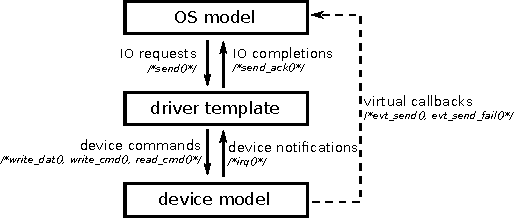
\includegraphics[width=0.85\linewidth]{imgs/actions.pdf}
    \caption{Input specifications for driver synthesis.  
    Labels in italics show interfaces from the running example
    (Figure~\ref{f:ex}).}\label{f:actions}
\end{figure}

The virtual interface between the device and the OS, shown with the dashed arrow in Figure~\ref{f:actions}, is used by the device model to notify the OS model about important hardware events, such as completion of I/O transactions and error conditions.  Methods of the virtual interface do not represent real runtime interactions between the device and the OS, but are used by the OS model to specify correctness constraints for the driver (see Section~\ref{s:virt}).

Finally, the driver template contains a partial driver implementation to be completed by \termite.  A minimal template consists of a list of driver entrypoints without implementation.  At the other extreme, it can provide a complete implementation, in which case \termite acts as a static verifier for the driver. By this we mean that it checks that the interactions between the driver software and the hardware ensure that all operating system requests are eventually fulfilled. It does not, for example, check for the absence of null pointer dereferences and similar defects that can be found by tools such as SLAM \cite{Ball_BKL_10}. In fact, \tsl is designed to express state machines, not arbitrary programs and such defects are not expressible. Of course, this also limits the drivers that can be expressed.

All specifications are written using the \termite Specification Language (\tsl).  In line with our goal of making synthesis as close to the conventional driver development workflow as possible, \tsl is designed as a dialect of C with additional constructs for use in synthesis.  The full specification of the \tsl language is given in Appendix~\ref{ch:tsl_ref}. We introduce relevant features of \tsl throughout this section.

We minimize the amount of work needed to develop specifications for every synthesized driver by maximizing the reuse of specifications.  In particular, \termite allows the use of existing device specifications developed by hardware designers in driver synthesis.  It does this by providing a compiler from the modelling language used for the existing specification to \tsl. This is explained in Section~\ref{sec:device_model}, however, we do not use this tool to generate the specifications used in the evaluation section (Section~\ref{s:eval}).

Furthermore, the OS specification for the driver can be derived from a generic specification for a class of similar devices (e.g., network or storage).  Thus we expect that additional per-driver effort will consist of: 
\begin{enumerate}
    \item inserting device-class callbacks in appropriate locations of the device model and 
    \item extending the OS specification to support device-specific features missing in the  generic OS specification.
\end{enumerate}

\subsection{Device model}
\label{sec:device_model}

The device model simulates the device operation at a level of detail sufficient to synthesize a correct driver for it.  To this end, it must accurately model external device behavior visible to software.  At the same time, it is not required to precisely capture internal device operation and timing, as these aspects are opaque to the driver.

Such device models are routinely developed by hardware designers for the purposes of design exploration, simulation, and testing. They are widely used by hardware manufacturers in-house~\cite{cofluent} and are available commercially from major silicon IP vendors~\cite{vp}.  These models are known as \emph{transaction-level models} (TLMs) (in contrast to the detailed register-transfer-level models used in gate-level synthesis)~\cite{Cai_Gajski_03}.  A TLM focuses on software-visible events, or \emph{transactions}, such as a write to a device register or a network packet transmission.

While the transaction-level modeling technology is relatively new, TLMs are already widely used by hardware manufacturers in-house~\cite{cofluent} and are available commercially from major silicon IP vendors~\cite{vp}.  We are optimistic that in the future open-source TLMs will become commonplace, since a TLM does not expose internal implementation details of the device and is therefore less likely to expose sensitive IP.

Existing TLMs created by hardware designers can be used with minor modifications (explained in Section~\ref{s:virt}) for driver synthesis.  Model reuse dramatically reduces the effort involved in synthesizing a driver and is therefore crucial to practical success of driver synthesis.  By reusing an existing model, we also reuse the effort invested by hardware designers into testing and debugging the model throughout the hardware design cycle, thus making driver synthesis less susceptible to specification bugs.  Finally, since TLMs are created early in the hardware design cycle, TLM-based driver synthesis can be carried out early as well, thus removing driver development from the critical path to product delivery.

TLMs are written in high-level hardware description languages like SystemC and DML\@.  In order to use these models in driver synthesis, we need to convert them to \tsl.  This translation can be performed automatically, and we are currently working on a DML-to-\tsl compiler.  Since this work is not yet complete, device models used in the experimental section of this paper are either manually translated from existing TLMs or written from scratch using TLM modeling style guidelines~\cite{dml_ug}.

Unfortunately, few TLMs are publicly available at the moment, which means that driver synthesis must be performed by  device vendors in-house.  However this is likely to change in the future.  A TLM does not expose internal implementation details of the device and is therefore not part of sensitive IP\@.  At the same time, there exist strong incentives for manufacturers to make device TLMs available to third-party vendors to test their software and hardware products for compatibility with the given device.

\subsubsection{Running example}

\begin{figure}
\begin{tsllisting}[name=ex]
/* Device model */
template dev 

    /* Device internal state */
    uint8 reg_dat, reg_cmd, reg_status = 0; (*@\label{f:ex_dev:l:reg_decls}@*)

    /* device commands */
    controllable void write_dat(uint8 v) { (*@\label{f:ex_dev:l:start_access}@*)
        reg_dat = v; 
    };

    controllable void write_cmd(uint8 v) { 
        reg_cmd = v; 
    };

    controllable uint8 read_cmd() { 
        return reg_cmd; 
    };

    controllable uint8 read_status() { 
        return reg_status; 
    }; (*@\label{f:ex_dev:l:end_access}@*)

    /* internal behavior */
    process ptx { (*@\label{f:ex_dev:l:start_xmit}@*)
        forever {
            wait (reg_cmd == 1); (*@\label{f:ex_dev:l:wait}@*)
            choice {(*@\label{f:ex_dev:l:atomic_start}@*)
                { 
                    os.evt_send(reg_dat); (*@\label{f:ex_dev:l:cb_succ}@*)
                    reg_status=0; 
                };
                { 
                    os.evt_send_fail(reg_dat);(*@\label{f:ex_dev:l:cb_fail}@*)
                    reg_status=1; 
                };
            };
            reg_cmd = 0; (*@\label{f:ex_dev:l:atomic_end}@*)
            /*drv.irq(); (see Section 4)*/(*@\label{f:ex_dev:l:irq}@*)
        };
    }; (*@\label{f:ex_dev:l:end_xmit}@*)
endtemplate
\end{tsllisting}
\caption{Trivial serial controller device specifications.}
\label{f:ex_dev}
\end{figure}

Figure~\ref{f:ex_dev} shows a fragment of a model of a trivial serial controller device used as a running example.  The fragment specifies the send logic of the controller, which allows software to send data characters over the serial line.  The model is implemented as a \tsl \emph{template}.  The template encapsulates data and code that manipulates the data, similar to a class in OOP.

The software interface of the device consists of data, command, and status registers declared in line~\ref{f:ex_dev:l:reg_decls}.  The registers can be accessed from software via the \src{write\_dat}, \src{write\_cmd}, \src{read\_cmd}, and \src{read\_status} methods (lines~\ref{f:ex_dev:l:start_access}--\ref{f:ex_dev:l:end_access}).  The \src{controllable} qualifier denotes a method that is available to the driver and can be invoked from synthesized code.

The transmitter logic is modelled in lines~\ref{f:ex_dev:l:start_xmit}--\ref{f:ex_dev:l:end_xmit}.  It is implemented as a \tsl \emph{process}.  A \tsl specification can contain multiple processes.  The choice of the process to run is made non-deterministically by the scheduler.  The process executes atomically until reaching a \src{wait} statement or a controllable placeholder (see below).

In line~\ref{f:ex_dev:l:wait}, the transmitter waits for a command, issued by the driver by writing value $1$ to the command register.  Upon receiving the command, it sends the value in the data register over the serial line.  The transmission may fail, e.g., due to a serial link problem.  The device signals transmission status to software by setting the status register to $0$ or $1$.  Finally, it clears the command register, thus notifying the driver the request has completed.

Internally, the transmitter circuit consists of a shift register and a baud rate generator used to output data on the serial line.  These details are not visible to software and are abstracted away in the model.  We use the non-deterministic \src{choice} construct to choose between successful transmission and failure, without modelling the details of serial link operation.  Successful and failed transmissions are modelled using\src{evt\_send} and \src{evt\_send\_fail} events, explained in Section~\ref{s:os}.

\subsection{OS model}\label{s:os}

The OS model specifies the API mandated by the OS for all drivers of the given type.  For example, any Ethernet driver must implement the interface for sending and receiving Ethernet packets.  A separate specification is needed for each supported OS, as different OSs define different interfaces for device drivers.

A high degree of specification reuse can be achieved by  creating a library of generic specifications for common types of drivers, e.g., network, storage, or serial drivers.  A generic specification describes the API mandated by the OS for all drivers of the given type.  For example, any Ethernet driver must implement the interface for sending and receiving Ethernet packets.  A separate generic specification is needed for each supported OS, as different OSs define different interfaces for device drivers.

Additionally, each particular device can support non-standard features, e.g., device-specific configuration options or transfer modes.  These features must be added as extensions to the generic OS specification in order to synthesize support for them in the driver.  \tsl supports such extensions in a systematic way via the template inheritance mechanism.  This is described in Appendix~\ref{ch:tsl_ref}.

\subsubsection{Running example}

\begin{figure}
\lstset{firstnumber=last}
\begin{tsllisting}[name=ex]
/* OS model */
template os 

    uint8 dat;
    bool inprogress, acked, success; (*@\label{f:ex_os:l:vars}@*)

    /* driver workload generator */
    process psend {
        forever {
            dat = *; /*randomise dat*/ (*@\label{f:ex_os:l:nondet}@*)
            inprogress = true;
            acked = false;
            drv.send(dat);
            wait(acked); (*@\label{f:ex_os:l:wait}@*)
        };
    };

    /* I/O completions */
    controllable void send_ack(bool status) { (*@\label{f:ex_os:l:ack}@*)
        assert (!inprogress && !acked && status == success);
        acked = true;
    };

    /* virtual callbacks */
    void evt_send(uint8 v) { (*@\label{f:ex_os:l:send_cb}@*)
        assert (inprogress && v==dat); (*@\label{f:ex_os:l:assert}@*)
        inprogress = false; (*@\label{f:ex_os:l:inprogress}@*)
        success = true; (*@\label{f:ex_os:l:success}@*)
    };

    void evt_send_fail(uint8 v) {
        assert (inprogress && v==dat);
        inprogress = false;
        success = false;
    };

    /* The goal */
    goal idle_goal = acked; (*@\label{f:ex_os:l:goal}@*)
endtemplate
\end{tsllisting}
\caption{Trivial serial controller driver specifications.}
\label{f:ex_os}
\end{figure}

Figure~\ref{f:ex_os} shows the operating system model. It is written in the form of a test harness that simulates all possible sequences of driver invocations issued by the OS\@.  The \src{os} template in Figure~\ref{f:ex_os} shows the OS model for our running example.  The main part of the model is the \src{psend} process.  At every iteration of the loop, it non-deterministically chooses an 8-bit value (line~\ref{f:ex_os:l:nondet}) and calls the \src{send} method of the driver, passing this value as an argument.  It then waits for the driver to acknowledge the transmission of the byte (line~\ref{f:ex_os:l:wait}) before issuing another request.  The driver acknowledges the transmission via the \src{send\_ack} callback (line~\ref{f:ex_os:l:ack}).  The callback sets the \src{acked} flag, which unblocks the \src{psend} process.

We keep the specification concise by modeling the state of the driver-OS interface, as opposed to the internal OS state and behavior.  For example, the \src{acked} variable (line~\ref{f:ex_os:l:ack}) serves to model the flow of data between the OS and the driver and is not necessarily present in the OS implementation.

\subsection{Connecting device and OS models}
\label{s:virt}

In addition to simulating I/O requests to the driver, the OS model also specifies the semantics of each request in terms of device-internal events that must occur in order to complete the requested I/O operation.  In our running example, after the OS invokes the \src{send} method of the driver and before the driver acknowledges completion of the request, the device must attempt to send the requested data over the serial line.  This requirement establishes a connection between the device and OS models and must be specified explicitly in order to enable \termite to generate a driver implementation that correctly handles the OS request.  Note that we only need to specify \emph{which} hardware events must occur, but not \emph{how} the driver generates them.

In order to develop such specifications, we need a way to refer to relevant state and behavior of the device from the OS model.  At the same time, in order to maximize specification reuse, we would like to keep the OS specification device-independent.  To reconcile these conflicting requirements, we introduce a \emph{virtual interface} between the device and OS model.  This interface consists of callbacks used by the device model to notify the OS model about important hardware events.  The virtual interface does not represent real runtime interactions between the device and the OS, but serves as part of the correctness specification.

We define a virtual interface for each class of devices.  Such \emph{device-class} interfaces are both device and OS-independent.  The device-class interface can be extended with additional device-specific callbacks as required to specify a driver for a particular device.

\subsubsection{Running example}

In our example, we define a device-class interface consisting of two virtual callbacks: \src{evt\_send} and \src{ev\_send\_failed}, invoked respectively when the device successfully transmits and fails to transmit a byte.  These callbacks are invoked in lines~\ref{f:ex_dev:l:cb_succ} and~\ref{f:ex_dev:l:cb_fail} of the device model.  The \src{evt\_send} handler is shown in line~\ref{f:ex_os:l:send_cb} of the OS model.  The assertion in line~\ref{f:ex_os:l:assert} specifies that the send event is only allowed to occur if there is an outstanding send request in progress and the value being sent is the same as the one requested by the OS\@.  We reset the \src{inprogress} flag to false in line~\ref{f:ex_os:l:inprogress}, thus marking the current request as completed; line~\ref{f:ex_os:l:success} sets the \src{success} flag to true, thus indicating that the transfer completed without an error.  The \src{evt\_send\_fail} handler is identical, except that it sets the \src{success} flag to false.  The flags are checked by the \src{send\_ack} method, which asserts that the driver is only allowed to acknowledge a completed request (\src{!inprogress}) that has not been acknowledged yet (\src{!acked}) and that the completion status reported by the driver must match the one recorded in the \src{success} flag.

In this example we use C-style assertions to rule out invalid system behaviors.  Assertions alone do not fully capture requirements for a correct driver behavior.  For example, a driver that remains idle does not violate any assertions.  Hence, we need to specify requirements for the driver to make forward progress.  We introduce such requirements into the model in the form of \emph{goal conditions}, that must hold \emph{infinitely often} in any run of the system.  For example, a goal may require that the driver is infinitely often in an idle state with no outstanding requests from the OS\@.  The OS can force the driver out of the goal by issuing a new I/O request.  To satisfy the goal condition, the driver must return to the goal state by completing the request.  Line~\ref{f:ex_os:l:goal} in Figure~\ref{f:ex_os} defines such a goal condition that holds whenever the \src{acked} flag is set, i.e., the driver has no unacknowledged send requests.

\subsection{Driver template}

\subsubsection{Running example}

\begin{figure}
\lstset{firstnumber=last}
\begin{tsllisting}[name=ex]
/* Driver template */
template drv 

    void send(uint8 v){ (*@\label{f:ex_drv:l:send}@*)
        ...; (*@\label{f:ex_drv:l:magic}@*)
    }; 

    /*
    void irq(){ (see Section 4) (*@\label{f:ex_drv:l:irq}@*)
        ...;
    }; 
    */
endtemplate
\end{tsllisting}
\caption{Trivial serial controller driver specifications.}
\label{f:ex_drv}
\end{figure}

Figure~\ref{f:ex_drv} shows the driver template for the running example consisting of a single \src{send} entry point invoked by the OS\@.  The ellipsis in line~\ref{f:ex_drv:l:magic} represent a location for inserting synthesized code and are part of \tsl syntax.  We refer to such locations as \emph{controllable placeholders}. 

\section{\tsl compiler}

In order to compute the most general driver strategy as a solution of a two-player game, we must first convert input \tsl specifications into a game automaton.  This conversion is performed by the \tsl compiler.

Real driver specifications have large state spaces, which cannot be feasibly represented by explicitly enumerating states.  Therefore, in \termite we represent games symbolically (Section~\ref{sec:symbolic_games}).  The state space of the game is defined in terms of a finite set of state variables $X$, with each state $s\in S$ representing a valuation of variables in $X$.  The \tsl compiler introduces a state variable for each \tsl variable declared in one of the input templates.  In addition, auxiliary state variables are introduced to model the current control location of each \tsl process.
        
We model controllable and uncontrollable actions as valuations of action variables $Y_c$ and $Y_u$.  Transition relations $\delta_c$ and $\delta_u$ are represented symbolically as formulas over state variables $X$, action variables $Y_c$ and $Y_u$, and next-state variables $X'$.  

The \tsl compiler splits the input specification into controllable and uncontrollable parts and translates them into controllable and uncontrollable transition relations respectively.  The controllable part is comprised of controllable methods that can be invoked by the driver.  The controllable transition relation $\delta_c$ is computed by rewriting controllable methods in the \emph{variable update form}.  Consider, for example, variable \src{reg\_dat} declared in line~\ref{f:ex_dev:l:reg_decls} in Figure~\ref{f:ex_dev}.  This variable is only modified by the \src{write\_dat} method in line~\ref{f:ex_dev:l:start_access}. The corresponding fragment of the controllable transition relation in the variable update form is
%$$
%\mathtt{reg\_dat' := (tag=write\_dat)~?~v : reg\_dat}
%$$
$$
\small
\begin{aligned}
    &reg\_dat' = \begin{cases}
                     v       , & \text{if } tag=write\_dat \\
                     reg\_dat, & \text{otherwise},
                 \end{cases}\\
\end{aligned}
$$
where $\mathtt{reg\_dat'}$ is the next-state variable representing the value of $\mathtt{reg\_dat}$ after the transition. A special $tag$ variable is used to identify the method being invoked. For example, the specification in Figure~\ref{f:ex_dev} has four controllable methods, so $tag$ can take one of the four values $write\_dat$, $write\_cmd$, $read\_status$ and $send\_ack$.  In addition, a separate variable is introduced for each argument of every controllable method ($v$ in this example). 

The uncontrollable part of the specification is comprised of \tsl processes, which model device and OS behavior.  We syntactically decompose each process into atomic transitions.  Recall that a process executes atomically until reaching a \src{wait} statement or a controllable placeholder.  Consider the \src{ptx} process in line~\ref{f:ex_dev:l:start_xmit} in Figure~\ref{f:ex_dev}.  The process is initially paused in the wait statement.  It is scheduled to run when the wait condition holds.  It executes the statements in lines~\ref{f:ex_dev:l:atomic_start}--\ref{f:ex_dev:l:atomic_end} atomically and stops again in line~\ref{f:ex_dev:l:wait}.  As part of this atomic transition, the process sets the \src{reg\_cmd} variable to 0 (line~\ref{f:ex_dev:l:atomic_end}).  This is the only uncontrollable transition that modifies this variable, hence the uncontrollable update function for this variable is defined as follows:
%$$
%\mathtt{reg\_cmd' := (reg\_cmd=1 \land pid=ptx)~?~0 : reg\_cmd}
%$$,
$$
\begin{aligned}
    &reg\_cmd' = \begin{cases}
                    0       , & \text{if } reg\_cmd=1 \land pid=ptx\\
                    reg\_cmd, & \text{otherwise},
                 \end{cases}\\
\end{aligned}
$$
where $\mathtt{pid}$ is an uncontrollable action variable that models the scheduler's choice of a process to run, and the $\mathtt{reg\_cmd=1}$ conjunct corresponds to the wait condition in line~\ref{f:ex_dev:l:wait}.
  
Finally, we need to generate the game objective $\Phi$.  In a symbolic representation of the game, goal and fair sets are specified as conditions over state variables that hold for each state in the set.  The \tsl compiler outputs a goal set $B_i$ for each goal declared in the input specification and a fair set $F_i$ for each \src{wait} statement.  The latter guarantees that every runnable process gets scheduled eventually.
        
In addition to goal conditions, a \tsl specification also contains assertions, which must never be violated.  We model assertions using an auxiliary boolean state variable $\varepsilon$, which is set to true whenever an assertion is violated and remains true forever after.  We add an extra constraint $\varepsilon=false$ to each accepting set $B_i$.  An assertion violation permanently takes the game out of $B_i$, and therefore can not occur in any winning run of the game.

\section{User-guided code generation}
\label{s:user-guided}

The set of input \tsl specifications is fed into the \termite synthesis engine, which then automatically computes the most general strategy for the driver.  Given a state of the system, the most general strategy determines the set of all valid driver actions in this state.  The most general strategy is used by the \termite code generator to produce a driver implementation in C in a user-guide fashion.

\subsection{Motivation}

Early versions of \termite implemented fully automatic code generation as their only mode of operation.  In many cases we found that the tool produced unsatisfactory code, which led to a series of improvements to the code generation algorithm, aimed to generate more compact, user-readable, and efficient implementations.  At the same time, we found that many aspects of what is perceived by developers as a good implementation are very hard to formalize, and, even when possible, the effort involved in such a formalization exceeds the effort needed to achieve the desired effect manually.

For example, the interrupt handler logic of most drivers follows the standard structure, where the driver checks every interrupt source in the order of its priority and invokes a separate handler function for every signaled interrupt.  Interrupt prioritization and functional decomposition are hard to synthesize automatically without manual guidance.

One might argue that structure and readability are not relevant for synthesized code.  In practice, however, if synthesized drivers are to make their way into Linux and other major OSs, they must follow standard coding guidelines adopted by these OSs and be amenable to manual code inspection.  Furthermore, human readable code is needed for quality assurance.  While automatic synthesis guarantees that the synthesized driver is correct with respect to input specifications, it does not protect against specification defects: despite our best effort to maximize specification reuse and follow good modeling practices, specification defects cannot be avoided altogether.  Hence, manual inspection remains an important way to eliminate driver bugs.

In summary, while there exists a potential for further improvement of automatic code generation algorithms, we believe that a truly practical driver synthesis tool must put the user in control of the resulting code and not enforce any particular code structure nor attempt to override user's design decisions.

\subsection{Workflow}

The \termite code generator GUI is similar to a traditional integrated development environment with two additional built-in tools: the \emph{generator} and the \emph{verifier}.  The generator works as advanced auto-complete that helps the user to fill the controllable placeholders inside the driver template with code.  At any point, the user can invoke the generator to synthesize a single statement or a complete block of code inside a controllable placeholder via a mouse click on the target code location.  The user can arbitrarily modify and amend the generated code.  However, the generator never modifies user code.  Instead it tries to extend it to a complete implementation, which is always possible provided that the existing code is consistent with the most general strategy.  The generator currently only allows synthesizing statements after the last control location within a branch.  However this restriction is not a conceptual one and will be lifted by ongoing development.

The verifier automatically and on the fly checks that the driver implementation, comprised of a mix of generated and manually written code, is consistent with the most general strategy, thus maintaining strong correctness guarantees that one would expect in automatically synthesized code.  The verifier symbolically simulates execution of the system, following the partial driver implementation created so far, and signals the user whenever it encounters a transition that violates the most general strategy.

In the first approximation, the generator algorithm is quite simple: given a source code location, it determines the set of possible system states in this location, picks an action for each state from the most general strategy and translates this action into a code statement.  In practice the algorithm uses a number of heuristics to produce compact and human-readable code.  In particular, whenever there exists a common action in all possible states in the given location, the algorithm produces straight-line code without branching. These heuristics are described in Section~\ref{sec:heuristic_codegen}.

\subsection{Running Example}

When running the generator on our running example, it automatically generates the code in Figure~\ref{f:ex_gen_send} for the \src{send} function (line~\ref{f:ex_drv:l:send} of the device template, Figure~\ref{f:ex_drv}):

\begin{figure}
\begin{tsllisting}
void send(uint8 v){
    dev.write_dat(v);
    dev.write_cmd(1);
    wait(dev.reg_cmd==0);
    if (os.success) {
        os.send_ack(true);
    } else {
        os.send_ack(false);
    };
};
\end{tsllisting}
\caption{Generated \code{send} function}
\label{f:ex_gen_send}
\end{figure}

This implementation correctly starts the data transfer by writing the value to be sent to the data register and setting the command register to $1$.  It then waits for the transfer to complete, which is signalled by the device by resetting the command register to $0$.  Finally, it acknowledges the completion of the transfer to the OS.

Note that the generated code refers to the \src{dev.reg\_cmd} and \src{os.success} variables.  These variables model internal device and OS state respectively and cannot be directly accessed by the driver.  This example illustrates an important limitation of \termite---it assumes a white-box model of the system, where every state variable is visible to the driver.  Ideally, we would like to synthesize an implementation that automatically infers the values of important unobservable variables.  In this case, the value of the command register can be obtained by the driver by executing the \src{read\_cmd} action.  Furthermore, the value of the \src{os.success} variable is correlated with the completion status of the last transfer, which can be obtained by reading the device status register.

While \termite currently cannot produce such an implementation automatically, it implements a pragmatic tradeoff that helps the user build and validate a correct implementation with modest manual effort.  The code generator warns the user that the auto-generated code accesses  private variables of the device and OS templates.  This prompts the user to provide a functionally equivalent valid implementation, replacing the \src{wait} statement with a polling loop and using the \src{read\_status} method to check transfer status, as shown in Figure~\ref{f:ex_man_send}.

\begin{figure}
\begin{tsllisting}
void send(uint8 v){
    dev.write_dat(v);
    dev.write_cmd(1);
    (*@{\bf\ttfamily while(dev.read\_cmd()==1){};}@*)
    if ((*@\bf\ttfamily dev.read\_status()@*)) {
        os.send_ack(true);
    } else {
        os.send_ack(false);
    };
};
\end{tsllisting}
\caption{Manually written \code{send} function}
\label{f:ex_man_send}
\end{figure}

The verifier automatically checks the resulting implementation and confirms that it satisfies the input specification.

Note that in this example we have synthesized code that correctly handles device errors.  This was possible, as our input device specification correctly captures device failure modes (namely, transmission failure) and our OS specification describes how the driver must report errors to the OS (via the \src{status} argument of the completion callback).

In principle, it is also possible to synthesize a driver implementation that handles device and OS failures \emph{not} captured in the specifications: since the synthesis tool knows all possible valid environment behaviors, it can easily detect invalid behaviors and handle them gracefully.  Automatic synthesis of such \emph{hardened} device drivers is a promising direction of future research.

The final step of the code generation process translates the synthesized driver implementation to C.  This is a trivial line-by-line translation.  We expect this translation to become unnecessary in the future as our ongoing work on the \tsl syntax aims to make the synthesized subset of \tsl a strict subset of C.

\subsection{Maintaining synthesized code~~} 
Device driver development is not a one-off task: following the initial implementation, drivers are routinely modified toimplement additional functionality, adapt to the changing OS interface or support new device features.

The user-guided code generation method naturally supports such incremental maintenance. Since \termite uses \tsl as both its input and output language;  a completely or partially synthesized driver can be given as input to \termite, along with modified versions of the device and OS models.

A typical maintenance task proceeds in three steps:

\begin{enumerate}
    \item First, the developer amends device and OS models to reflect the new or changed functionality.  
    \item Second, they add new methods to the previously synthesized driver, if necessary, and replace existing driver code that is expected to change with a controllable  placeholder.  
    \item Finally, the user runs \termite to synthesize code for all controllable placeholders.  
\end{enumerate}
        
\termite treats all existing driver code as part of the uncontrollable environment.  Hence, if some of the old code is incorrect in the context of the new specifications, this will lead to a synthesis failure, and counterexample-based debugging is used to identify the faulty code, as described in Section~\ref{s:debug}.

\subsubsection{Running Example}

As an example, we synthesize a new version of the driver for our running example assuming a more advanced version of the serial controller device that uses interrupts to notify the driver on completion of a data transfer.  The new device model is obtained by uncommenting line~\ref{f:ex_dev:l:irq} of the device model in Figure~\ref{f:ex_dev}, which invokes the interrupt handler method of the driver after each transfer.  The driver template (Figure~\ref{f:ex_drv}) is extended with the \src{irq} method (line~\ref{f:ex_drv:l:irq}).  We use the previously synthesized implementation of the \src{send} method, but manually remove the last two lines, which implement polling, as we want the new implementation to use interrupts instead:

\begin{tsllisting}
void send(uint8 v){
    dev.write_dat(v);
    dev.write_cmd(1);}
\end{tsllisting}

Finally, we run \termite on the resulting specifications and use the generator to automatically produce the following implementation of the new \src{irq} method:

\begin{tsllisting}
void irq(){
    if (os.success) {
        os.send_ack(true);
    } else {
        os.send_ack(false);
    };}
\end{tsllisting}

As before, we manually replace the if-condition in the first line with

\begin{tsllisting}
if (dev.read_status())
\end{tsllisting}

This example illustrates how \termite supports incremental changes to the driver by reusing previously synthesized code, while maintaining strong correctness guarantees.

\subsection{Instrumenting synthesized code~~} 
\termite does not automatically instrument synthesized code for debugging, logging, accounting, etc.  However, the user can add such instrumentation manually.  \termite interprets such code as no-ops and, as with any manual code, never makes any modifications to it.

\section{Heuristic code generation}
\label{sec:heuristic_codegen}

Termite acts as an advanced auto-complete by suggesting lines of code for the driver. These suggestions are obtained using the symbolic strategy generated in the synthesis phase. Termite keeps track of the possible set of states that the system may be in at each line of code in the graphical IDE and uses this along with the strategy to generate a suggestion. 

Generating a winnng move from an individual state is straightforward. All one has to do is look up the state in the strategy relation and pick any winning label related to that state. Termite's code generator, however, deals in sets of states - the set of states which the system may be in at a particular line - which complicates matters considerably. For example, although every state in the set is winning (an invariant that the code generator enforces), there might not exist a single label that is winning for all of these states. In this case, the code generator uses smarter methods for picking labels or possibly falls back to spliting the current state set in two, as described in the following sections.

\subsection{Straightford label picking}

In the simplest case, there exists a winning action that is available from all states within the current line's state set (denoted $stateSet$). This action will cause all states in $stateSet$ to transition to a state closer to the goal, guaranteeing that if we keep choosing actions in this way we will eventually force execution into the goal. We compute the set of such winning actions using the formula in Equation~\ref{eqn:simple_strat}. 

\begin{equation}
\forall s. \: stateSet \rightarrow strategy
\label{eqn:simple_strat}
\end{equation}

This returns the set of labels which are part of the strategy for all states in the current state set. If the set is not empty, the Termite IDE the picks one of these at random as the autocompletion suggestion. If it is empty, the Termite IDE falls back to the more computationally expensive heuristic described in the next section.

\subsection{Smarter label picking}

While the above heuristic is straightforward and cheap, is it often unsatisfactory in practice. As an example, consider a current state set containing two states: $s_1$ and $s_2$. Suppose there is no label which is in the winning strategy for both states, but there is a label in the winning strategy for $s_1$ and it does not take $s_2$ further away from the goal. Such an action is a good candidate for an auto completion, however it will not be found by the first heuristic.

Our more general label picking algorithm works as follows: we find the greatest distance (N) of any state in $stateSet$ from the goal and then we look up two sets (which were computed and saved during synthesis).

\begin{itemize}
    \item the set of states at distance $N$, denoted $win_N$,
    \item and, the set of states at distance $N-1$, denoted $win_{N-1}$.
\end{itemize}

We define three constraints on the label, all computable symbolically, and pick a label that satisfies all three constraints by taking their conjunction, also symbolically.

When played, the label must:

\begin{itemize}
    \item keep execution in $win_{N-1}$ for states within $stateSet \cap win_{N-1}$, and
    \item keep execution in $win_N$ for states within $stateSet \cap win_N$, and
    \item take at least one state in $win_N$ into $win_{N-1}$.
\end{itemize}

These requirements ensure that each time a label is picked in this way, the number of states at the furthest distance to the goal decreases and eventually becomes zero as the number of abstract states in finite, in turn decreasing the maximum distance to the goal, $N$. Thus, repeatedly picking actions in this way ensures that we eventually get to the goal and is therefore a sound method of picking auto completions. Note that even though execution is guaranteed to reach the goal, the label picked may not be part of the strategy for all states in $stateSet$.

\subsection{Splitting states}

Lastly, suppose that there is no action found by the first two heuristics. In this case we recursively split $stateSet$ by finding a subset $a \subset stateSet$ from which there is a winning action for all of $a$ and splitting this out in C code using an \emph{if-statement}. What remains of $stateSet$ is recursively split enough times that there is a suitable label to play from each partition. This is guaranteed to eventually happen because $stateSet$ in finite. 

We describe how the condtion for this if-statement is computed. There exists at least one winning label from each state in the current set, as they are all winning. However, there does not exist a single label which is winning for all states in the current set. Our heuristic to find a subset of $stateSet$ for which there does exist such a label is as follows:

\begin{enumerate}
    \item Enumerate labels that are winning in some state in $stateSet$.
    \item Compute the set where each label is part of the strategy.
    \item Compute a small condition over state variables that distinguishes this set from the rest of $stateSet$.
    \item Choose the condition that is the simplest and return this and the corresponding lablel.
\end{enumerate}

\subsubsection{Enumerating winning labels}

In practice, the first step is infeasible, however. Games in Termite have labels over 100 bits in size so this would require enumerating over $2^{100}$ labels. However, many of these labels are equivalent as certain combinations of bits are dont-care. We use the $availableLabels$ algorithm (Algorithm~\ref{alg:available_labels}) to enumerate labels that are equivalent given the current set and transition relation.

This algorithm invokes two other algorithms: $genPair$ (Algorithm~\ref{alg:gen_pair}) and $enumerate$ (Algorithm~\ref{alg:enumerate}), both of which deserve some explanation. 

$genPair$, given two sets of variables ($X$ and $Y$) and a relation, extracts a single valuation of $X$ from the relation, determines the set of valuations of $Y$ that are related to and then determines the set of valuations of $X$ that relate to exactly this set. 

$enumerate$, given two sets of variables ($X$ and $Y$) and a relation repeatedly extracts pairs from the relation using $genPair$, erasing the $X$ valuations from the relation each time so that they are not chosen again. It computes a set of pairs of sets of $X$ and $Y$ valuations that are related to exactly the other element of the pair.

Finally, $availableLabels$ uses $enumerate$ to enumerate labels with different behaviours in the current $stateSet$. It does this by restricting the transition relation to transitions that originate from states in $stateSet$ and treating this as a relation between $\langle s, s' \rangle$ and $l$. This works because equivalent labels will result in the same $\langle s, s' \rangle$ relation, i.e.\ the same state transition, thus calling $enumerate$ with this relation and these variables will enumerate equivalent labels.

\begin{algorithm}
\begin{algorithmic}

\Function{GenPair}{$x$, $y$, $rel$}
    \State $xMinterm \gets \Call{extractMinterm}{\exists y. \: rel}$
    \State $img      \gets \Call{substitute}{rel, xMinterm}$
    \State $genX     \gets \forall y. \: reg \leftrightarrow img$
    \State\Return $\langle genX, img \rangle$
\EndFunction

\end{algorithmic}
\label{alg:gen_pair}
\end{algorithm}

\begin{algorithm}
\begin{algorithmic}

\Function{Enumerate}{$x$, $y$, $rel$}
    \State $result = []$
    \While{$rel \neq False$}
        \State $\langle genX, img \rangle \gets \Call{genPair}{x, y, rel}$
        \State $result \gets result \oplus \langle genX, img \rangle$
        \State $rel \gets res \land \neg genX$
    \EndWhile
    \State\Return $result$
\EndFunction

\end{algorithmic}
\end{algorithm}

\begin{algorithm}
\label{alg:enumerate}
\begin{algorithmic}

\Function{availableLabels}{$s, u, l, s', strategy, stateSet$}
    \State $winning \gets \exists \: s \: u \: s'. \: strategy \land stateSet$
    \State\Return$\Call{enumerate}{l, s \cup s', \delta \land stateSet \land winning}$
\EndFunction

\end{algorithmic}
\label{alg:available_labels}
\end{algorithm}

\subsubsection{Computing the condition}

We compute a condition over state variables that distinguishes the states where the label is winning from the rest using the $liCompaction$ function. This function, provided by the CUDD library, minimises a condition BDD given a care set so that it returns the correct value within the care set and is undefined otherwise. Our condition BDD is the set of states from the winning label is available and our care set is $currentState$. Since we are only applying the if condition in one of the states in $currentState$, this is the only set where it needs to be accurate. 

We found that a good heuristic is to choose the label which results in the simplest if condition, where a simple condition has a small BDD representation. The size of a BDD can be conveniently calculated using the function $dagSize$ from the CUDD library. 

\section{Counterexample guided debugging}
\label{s:debug}

An important practical issue in game-based synthesis is the complexity of diagnosing synthesis failures due to defects in the input specifications.  In the event that \termite fails to solve the game, the user needs to trace the failure back to the specification defect.  However, the failure does not carry any information about the defect, which makes the problem harder to resolve.

In \termite we propose a new approach to troubleshooting synthesis failures based on the use of \emph{counterexample strategies}.  A counterexample strategy is a strategy on behalf of the environment that prevents the driver from winning the game.  It is obtained by solving the \emph{dual game}, where, in order to win, the environment must permanently force the game out of one of the goal regions.  A winning strategy in the dual game is guaranteed to exist whenever solving of the primary game fails.

By exploring the counterexample strategy, the user can identify the defect in the input specification.  This is similar to the use of counterexamples in software verification, where for each discovered bug the verification tool generates a counterexample trace that triggers the bug.  However, a counterexample strategy cannot in the general case be represented by a single execution trace, as the choice of spoiling moves for the environment depends on the actions performed by the driver.

In order to detect and fix the defect in an input specification, the driver developer relies on their  understanding of the OS and device logic.  The role of the counterexample strategy is to guide the developer towards the defect.  To automate this process, we developed a powerful visual debugging tool that allows the user to interactively simulate intended driver behavior and observe environment responses to it.  The user plays the game on behalf of the driver, while the tool responds on behalf of the environment, according to the counterexample strategy.
 
In a typical debugging session, the debugger, following the counterexample strategy, generates a sequence of requests that are guaranteed to win against the driver.  The user plays against these requests by specifying device commands that, they believe, represent a correct way to handle the request.  Since this sequence of requests \emph{cannot} be handled correctly given the current input specification, at some point in the game the user runs into an unexpected behavior of one of the players, e.g., one of the user-provided commands does not change the state of the device as expected or the environment performs an uncontrollable transition that violates an assertion.  Based on this information, the user can revise the faulty specification.

At every step of the interactive debugging session, the debugger either chooses a spoiling uncontrollable action based on the counterexample strategy or, if the system is inside a controllable placeholder, allows the user to choose a controllable action to execute on behalf of the driver.  In the former case the spoiling uncontrollable action corresponds to a transition in one of the \tsl processes.  The user can explore this transition by stepping through it, exactly as they would in a conventional debugger.  In the latter case, the user provides the action that they would like to perform by typing and executing corresponding code statements.

The tool supports a number of features aimed at making the debugging process as simple as possible for the user. We mention two of them here: 
\begin{itemize}
    \item First, the debugger interactively prompts actions available to the driver at each step.  
    \item Second, the debugger keeps the entire history of the game and allows the user to go back to one of previously explored states and try a different behavior from there.
\end{itemize}

\section{Limitations}\label{s:limitations}

The core of a device driver entails translating I/O requests from the OS into sequences of low-level device commands and responses. We focus on synthesizing driver logic that performs these functions, and this is where game-based synthesis really shines, as it helps to implement tedious and error-prone logic with minimal manual effort and without bugs. However, there are several real world aspects of device driver creation that are not handled as gracefully by the game based approach.

In Section~\ref{s:user-guided}, we described one limitation of \termite, namely the lack of support for grey-box synthesis.  In this section we discuss other limitations, which, we hope, will help define the agenda for continuing research in driver synthesis.

\subsection{Direct Memory Access}

Most importantly, \termite does not currently support automatic synthesis of direct memory access (DMA) management code.  Many modern devices transfer data directly to and from main memory, where it is buffered in data structures such as circular buffers and linked lists.  These data structures can have very large or infinite state spaces and cannot be easily modeled within the finite state machine-based framework of \termite.  Efficient synthesis for DMA requires enhancing the synthesis algorithm to use a more compact representation of DMA data structures, which is the focus of our ongoing research.  At this time, code for manipulating DMA data structures must be written manually.  This code is not interpreted or verified by \termite.  For example, we use this approach to synthesize a DMA-capable IDE disk driver (Section~\ref{s:eval}).

\subsection{Boilerplate Code}

Device drivers in modern OSs contain a significant amount of boilerplate code that is not directly related to the task of controlling the device.  This includes binding the driver to I/O resources (memory mapped regions, interrupts, timers), registering the driver with various OS subsystems, allocating DMA memory regions, creating sysfs entries, etc.  While much of this functionality could be synthesized within the game-based framework, we do not believe that this is the correct approach.  Previous research has demonstrated that this boilerplate code can be generated in a principled way from declarative specifications of the driver's requirements and capabilities~\cite{Spear_RHHL_06}.  This technique has lower computational complexity than game solving and better captures the essence of the task.  A practical driver synthesis tool can combine game-based synthesis of the core driver logic responsible for controlling the device with declarative synthesis of boilerplate code.  As a result, the current version of \termite assumes this boilerplate code is written manually as a wrapper around the synthesized driver.

\subsection{Concurrency}

Drivers execute in a concurrent OS environment and must handle invocations from multiple threads, as well as asynchronous hardware interrupts.  We separate synthesis for concurrency into a separate step.  Drivers synthesized by \termite are correct assuming a sequential environment, where driver entry points are invoked atomically.  The resulting sequential driver is then processed by a separate tool that performs a sequence of transformations of the driver source code, which preserve the driver's sequential behavior, while making the driver thread-safe.  Such transformations include adding locks around critical code sections, inserting memory barriers, and reordering instructions to avoid race conditions.  Concurrency synthesis is still work in progress and is not the subject of this thesis.  Preliminary results are published in~\cite{Cerny_HRRT_13, Cerny_HRRT_14}.

\subsection{Real time synthesis}

\termite does not explicitly support specification and synthesis of timed behaviors.  Instead, it uses a pragmatic approach that allows it to synthesize time-sensitive behavior without having to explicitly reason about time.  To this end, \termite conservatively approximates timed operations by fairness constraints: it ignores the exact duration of each device operation, but keeps the knowledge that the operation will complete \emph{eventually}, and synthesizes a driver that waits for the completion.  \termite is also able to handle time-out conditions, modeled as external events.  However, at this time it is not capable of generating device drivers for hard real-time systems, where the driver must guarantee completion of I/O operations by a certain deadline.

\section{Implementation}

We implemented all components of the Termite toolkit, including the TSL compiler, the game solver, the counterexample debugger, the user-guided code generator, and the TSL-to-C compiler, in the Haskell programming language.  Our implementation uses the CUDD BDD library for efficient symbolic manipulations over boolen relations, and the Z3 SMT solver for satisfiability queries over the theory of bit vectors, as described in~\cite{Walker_Ryzhyk_14}.  Termite is publicly available under the BSD license and can be downloaded from the project website \texttt{\url{http://termite2.org}}. The version of \termite presented here consists of 30,000 lines of code.  The estimated overall project effort is 10 person years. 

\section{Evaluation}
\label{s:eval}
We evaluate \termite by synthesizing drivers for eight I/O devices.  Specifically, we synthesized drivers for a UVC-compliant USB webcam, the 16550 UART serial controller, the DS12887 real-time clock, and the IDE disk controller for Linux, as well as bare metal drivers (which, for example, would run on seL4~\cite{Klein_EHACDEEKNSTW_09}) for I2C, SPI, and UART controllers on the Samsung exynos 5 chipset\footnote{At the time of writing, the exynos drivers have not yet been tested due to hardware availability issues; however we confirmed via manual inspection that they implement the same device control sequences as existing manually developed drivers.} and SPI controller on the STM32F10 chipset.  With the exception of the IDE disk, these devices are representative of peripherals found in a typical embedded platform, such as a smartphone.  Our synthesized drivers implement data transfer, configuration and error handling.  The main barrier to synthesizing drivers for more advanced devices, e.g., high-performance network controllers, is the current lack of support for synthesis of DMA code in the current version of \termite.  

\subsection{Modelling complexity} 
Models of UART and DS12887 devices were developed based on existing publicly available device models~\cite{ds12887, uart}.  Models of other devices were derived from their vendor-provided documentation, following standard TLM modeling guidelines~\cite{dml_ug}.  OS models for the relevant device classes were created based on Linux kernel documentation and source code.  

Table~\ref{t:size} summarises the size, in lines of code, of device and OS models in our case studies.  Developing a complete set of specifications for each driver took approximately one week, of which only one to three days were spent building the models and the rest of the time was spent studying device and OS documentation.  This efficiency can be attributed to the choice of the right level of abstraction and modeling language.  In particular, the use of transaction-level device modeling abstracts away complicated internal device machinery by focusing on high-level events relevant to driver synthesis, while the \tsl language allows modeling the driver environment using standard programming techniques, as illustrated by our running example.

\begin{table}
    \begin{minipage}{\linewidth}
    \center
    %\begin{tabular}{|p{0.15\linewidth}|p{0.15\linewidth}p{0.15\linewidth}|p{0.15\linewidth}p{0.15\linewidth}|}
    \begin{tabular}{|l|c|c|c|c|}
        \hline
%        & \multicolumn{4}{|c|}{size (lines of code)} \\
%        \cline{2-5}
        & \multicolumn{2}{|c|}{input spec} & \multicolumn{2}{c|}{driver} \\
        \cline{2-5}
                     & OS  & device & synthesized & native \\
        \hline
        \hline
        webcam       & 102 & 385    & 113         & 307 \\
        16450 UART   & 122 & 167    & 74          & 261 \\
        exynos UART  & 128 & 252    & 37          & 166 \\
        STM SPI      & 73  & 244    & 24          & 64  \\
        exynos SPI   & 88  & 239    & 40          & 183 \\
        exynos I2C   & 146 & 180    & 79          & 211 \\
        RT clock     & 118 & 252    & 84          & 183 \\
        IDE          & 188 & 480    & 94\footnote{Excluding 36 lines of manually written code that manipulates the DMA descriptor table.} & 474 \\
        \hline
    \end{tabular}
    \end{minipage}
    \caption{Size (in lines of code) of input specifications and of synthesized and equivalent manually written drivers.}
    \label{t:size}
\end{table}

Interestingly, we found the most error-prone step in developing specifications for driver synthesis to be defining correct relative ordering of OS-level and device-level events with the help of the virtual interface (Section~\ref{s:virt}).  Na\"ive specifications tend to be either too restrictive, leading to synthesis failures, or too liberal, leading to incorrect synthesized drivers. As we gained more experience synthesizing different types of drivers, we identified common modeling patterns that help avoid errors in virtual interface specifications.  

As a common example, most virtual interfaces contain callbacks that signal a change to one of the device configuration parameters, e.g., transfer speed, parity, etc.  A na\"ive OS model may only allow such a callback to be triggered when the OS has requested a change to the corresponding device setting.  However, many devices only allow setting multiple configuration parameters simultaneously, so that setting any individual parameter triggers multiple callbacks, thus making the specification non-synthesizable.  The problem can be rectified by changing the device specification to only trigger callbacks if the new value of the parameter is different from the old one; however this bloats the device model due to the extra checks.  A better solution, used in all our models, is to design the OS specification to allow configuration callbacks to be triggered at any time, provided that the new value of the parameter is equal to the last value requested by the OS. 

\subsection{Synthesis time} 
Table~\ref{t:perf} summarises the performance of the \termite game solver in our case studies.  The second column of the table characterises the complexity of the two-player game constructed by the \tsl compiler from the input specifications in terms of the number of states variables and the total number of bits in these variables.  The third column shows the number of iterations of the abstraction refinement loop required to solve the game.  The next column shows the size of the abstract game at the final iteration, in terms of the number of predicates in the abstract state space of the game.  These results demonstrate the dramatic reduction of the problem dimension achieved by our abstraction refinement method.  The second-last column shows that the \termite game solver was able to find the most general winning strategy within a few minutes in all case studies.

\begin{table}
    \center
    \begin{tabular}{|l|ccccc|}
        \hline
                       & \multirow{2}{*}{vars(bits)} & refine- & predi- & synt.     & verif.   \\
                       &                             & ments   & cates  & time (s)  & time (s) \\
        \hline
        \hline
        webcam         & 128 (125565)                & 47      & 192    & 215       & 794 \\
        16450 UART     & 81  (407)                   & 65      & 128    & 210       & 464 \\
        exynos UART    & 80  (1185)                  & 54      & 111    & 645       & 82 \\
        STM SPI        & 68  (389)                   & 29      & 63     & 67        & 31 \\
        exynos SPI     & 83  (933)                   & 31      & 72     & 25        & 44 \\
        exynos I2C     & 65  (303)                   & 21      & 56     & 45        & 96 \\
        RT clock       & 92  (810)                   & 25      & 74     & 56        & 127 \\
        IDE            & 114 (1333)                  & 42      & 105    & 285       & 778 \\
        \hline
    \end{tabular}
    \caption{Performance of the \termite game solver.}
    \label{t:perf}
\end{table}

We compared the performance of the \termite game solver against a state-of-the-art abstraction refinement algorithm for games~\cite{Alfaro_Roy_07} as well as against the standard symbolic algorithm for solving games without abstraction~\cite{Piterman_PS_06}.  In all case studies, the \termite solver was the only one to find a winning strategy within a two-hour limit.  We refer the reader to~\cite{Walker_Ryzhyk_14} for a more detailed performance analysis of the \termite synthesis algorithm.

The final column of Table~\ref{t:perf} shows the time that it took \termite to verify a complete driver.  Recall that the \termite synthesis algorithm doubles as a verification algorithm and can be used to verify drivers written in \tsl.  We used complete synthesized drivers containing a combination of manual and automatically generated code as inputs to \termite.  We have been able to successfully verify all of our drivers.  We also experimented with introducing faults to synthesized drivers.  \termite was able to detect these faults and produce correct counterexample strategies.  In most cases verification took longer than synthesis.  The reason for this is that \termite has not yet been optimized for verification workloads.  This is one area for future improvement.

%\termite is the first synthesis tool based on abstraction 
%refinement, so we cannot compare it against other 
%abstraction-based algorithms.  We benchmark \termite against a 
%highly optimized implementation of the state of the art algorithm 
%for solving GR-1 games (without abstraction) by Piterman et 
%al.~\cite{Piterman_PS_06}.  This algorithm was not able to solve 
%any of our case studies within a two-hour time limit.  We 
%therefore produced a simplified version of the IDE case study with 
%only 75 state bits (instead of 1333 in the original 
%specification), which the Piterman et al. algorithm solved in 
%57 minutes.  For comparison, \termite solved this simplified 
%example in under 1 second.

\subsection{User-guided code generation and debugging} 
We evaluate the key contribution of this paper, namely the user-guided debugging and code generation technique.  Each line of code in a \termite-generated driver originates from one of three sources: it can be 
\begin{enumerate} 
    \item synthesized automatically by the tool, 
    \item developed offline and given to \termite as part of the driver template, or 
    \item added or modified by the user during an interactive code generation session.  
\end{enumerate}
A perfect synthesis tool, capable of generating a complete driver fully automatically while producing code that meets all non-functional requirements, would eliminate the need for manual code altogether.  We do not believe that such a tool is feasible in the near future.  We therefore explore the tradeoffs that arise when using our current, imperfect, tool.  In particular, we would like to empirically characterize situations when the user can rely on the synthesizer to automatically produce near-optimal code, and when they are better off completely or partially implementing certain functionality manually.  These tradeoffs are likely to change as the tool improves.

Based on our experience so far, automatic synthesis is most helpful in generating code that performs device configuration or starts a data transfer.  This code may involve a long sequence of commands to the device, which must be issued in the right order and with correct arguments.  The synthesis algorithm of \termite proved more effective at doing this than human developers, producing correct code that only requires minimal cosmetic changes in most cases.  For example, Figure~\ref{f:screenshot_write} shows a screenshot of \termite with a synthesized implementation of the IDE driver \src{write()} function, which starts a data transfer to the device.  The function writes request parameters into appropriate device data registers and sets bit fields in command registers to prepare the device for data transfer.  One deficiency in this auto-generated implementation is that it uses absolute values instead of symbolic constants for bit fields.

As another example of suboptimal synthesized code, consider the following synthesized fragment:

\vspace{5mm}
\begin{tsllisting}
void packet_received() {
    if (((packet_data[9:9] == 1) && (packet_data[14:14] == 1))) {
        os.ack_packet(1,1,packet_data[16:32]);
    } else if ((dev.packet_data[9:9] == 1)) {
        os.ack_packet(1,0,packet_data);
    } else if ((dev.packet_data[14:14] == 1)) {
        os.ack_packet(0,1,packet_data[16:32]);
    } else {
        os.ack_packet(0,0,packet_data[16:32]);
    };
};
\end{tsllisting}
\vspace{3mm}

which can be replaced by an equivalent one-liner:

\vspace{5mm}
\begin{tsllisting}
os.ack_packet(packet_data[9:9],
    packet_data[14:14],packet_data[16:32]);
\end{tsllisting}
\vspace{5mm}

\noindent While both issues can, and will, be addressed by an improved code generation algorithm, our experience shows that unaccounted corner cases will arise occasionally.  Therefore, the ability to manually modify synthesized code without sacrificing correctness is crucial for a practical synthesis tool.

Limitations of \termite are most noticeable in synthesizing interrupt handler code responsible for processing I/O completions.  This involves querying device state to determine which operations completed and with what status, reporting results to the OS, and clearing interrupt status registers.  Since \termite does not support grey-box synthesis, it can not generate this code automatically and instead produces code that directly accesses device-internal state (see Section~\ref{s:user-guided}).  \termite correctly reports such situations and allows the user to mitigate them by manually editing synthesized code.  In practice, however, we found it easier to develop most of the interrupt handler logic offline, as part of the driver template, and rely on \termite to (a) establish correctness of this code and (b) extend it to a complete implementation.

\begin{figure}
    \center
    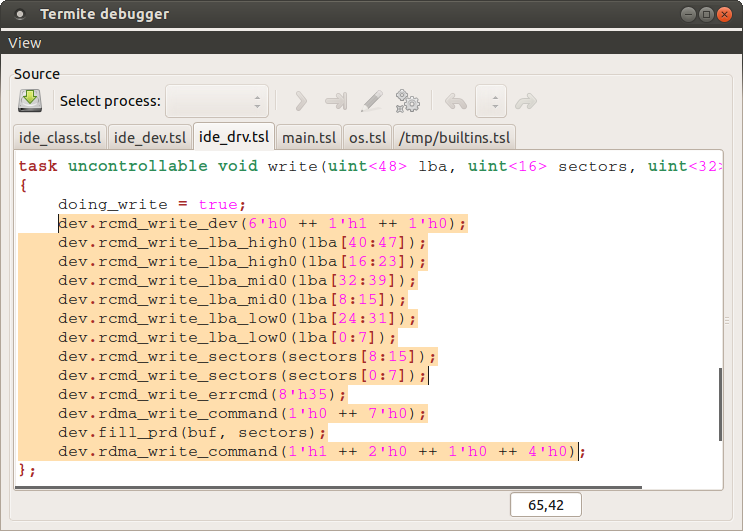
\includegraphics[width=\linewidth]{imgs/screenshot_write.png}
    \caption{Screenshot of \termite with a synthesized implementation of the IDE driver.  Automatically generated code is highlighted.}
    \label{f:screenshot_write}
\end{figure}

In our case studies, 60\% to 90\% of the code was generated fully automatically, with the rest of the code produced in a user-guided fashion.  Once an initial version of device and OS specifications was ready, it took us several hours to generate the driver implementation for each of our case studies.  Three quarters of this time was spent debugging the input specifications, with the rest of it spent generating driver source code with the help of the user-guided code generation GUI.

We found counterexample-driven debugging to be crucial to the productivity of synthesis-based development.  Before the debugger was available, we had to rely on code inspection to identify defects in the input specifications, which proved to be a frustrating and unpredictably long process.  The \termite debugger streamlines this process, giving us the confidence that any failure can be localised by following well-defined steps.  A typical debugging session takes a few minutes and involves entering only a few commands manually before the defect is localised. 

%We found the incremental approach to debugging and synthesis to 
%be the most effective.  Incremental synthesis 
%
%synthesise a single driver function or a small group of related 
%functions before adding m
%
%This is achieved by disabling invocations of all but one I/O 
%operations in the OS model. 
%
%Incremental synthesis

%In all case studies, we have been able to achieve human-readable 
%code structure that one would expect in a manually developed 
%driver.  60\% to 90\% of the code was generated fully 
%automatically and did not require any manual changes.  The rest of 
%the code was produced in a user-guided fashion, as described in 
%Section~\ref{s:user-guided}.  Human involvement was required for 
%three reasons.  First, it was necessary to get around the 
%white-box assumption, causing automatically generated code to 
%access variables outside the syntactic scope of the driver, as 
%explained in Section~\ref{s:user-guided}.  Second, it was used to 
%enforce a particular preferred implementation among several 
%functionally equivalent alternatives.  A common example of such a 
%situation, illustrated in Section~\ref{s:user-guided}, is 
%implementing I/O completions using interrupts instead of polling.  
%Finally, we relied on manual intervention to improve the structure 
%of synthesized code to make it compliant with the standard Linux 
%driver structure.

\subsection{Size of synthesized code} 
The last two columns of Table~\ref{t:size} compare the size of synthesized drivers to existing manually developed drivers.  Synthesised drivers are significantly more compact than conventional drivers for two main reasons.  First, as explained in Section~\ref{s:limitations}, we only synthesize the driver logic directly responsible for controlling the device.  Conventional drivers typically contain a large amount of boilerplate code managing various OS resources.  We believe that this code can and should be synthesized using complementary techniques.  At the moment we implement this functionality manually as a wrapper around the synthesized driver. 

Second, conventional device drivers are often designed to support multiple similar devices with slightly different interfaces and capabilities.  This leads to code bloat, as the driver must implement multiple versions of various operations, as well as logic to dynamically discover device capabilities and choose the right implementation to use.  In contrast, every \termite driver supports one specific device model with a fixed set of features.  Drivers for similar devices can share common specification code, but are synthesized as separate source code modules.  This approach leads to simpler code and is preferable for platforms with a fixed set of peripheral devices, such as smartphones, where shipping drivers that support only the required devices enables smaller system image.
  
\subsection{Specification reuse}  
Our specification methodology ensures mutual independence of device and OS specifications, and thus facilitates their reuse.  We have not yet carried out a substantial evaluation of such reuse; however we report our limited experience based on synthesizing two SPI drivers for the seL4 OS\@.  The corresponding OS specification was initially developed during the work on the SPI driver for the exynos chipset.  It was later used to synthesize a driver for the STM32F10 chipset.  We were able to reuse most of the original specification.  Minor changes (8 lines of code) were required in the part of the specification describing configuration functionality of the driver, since the STM SPI controller supports a number of ad hoc transfer modes.  We expect to observe similar pattern for other devices and operating systems: generic OS specifications can be reused with localized, device-specific changes required to support non-standard device features.

\subsection{Performance of synthesized drivers} 
Our synthesized drivers implement effectively identical device control logic to their conventional counterparts and therefore have similar performance.  We benchmarked the USB webcam driver, which is the most performance-critical one among our case studies.  We measured CPU load and data throughput generated by the conventional and synthesized drivers for varying bitrates.  We obtained identical results, modulo measurement errors, for both drivers in all cases.

